\section{Performance}The HTCC is one of the major CLAS12 systems used in all experiments with electron beam. The most important aspects of the HTCC performance to be addressed are providing good timing, high electron detection efficiency, high signal strength, and high rejection factor of charged pions. All this parameters are critical for the quality of the data obtained in experiments since the detector in combination with the forward calorimeter provides a fast trigger signal for CLAS12. 

As shown in subsection 6 the MC prediction has an efficiency of $\approx$100\% at. In the Fig.\ref{fig:RAFO_2GeV}. is presented the experimentally measured electron detection efficiency for elastically scattered electrons at 2 GeV. 

\begin{figure}[!ht]
    \centering
    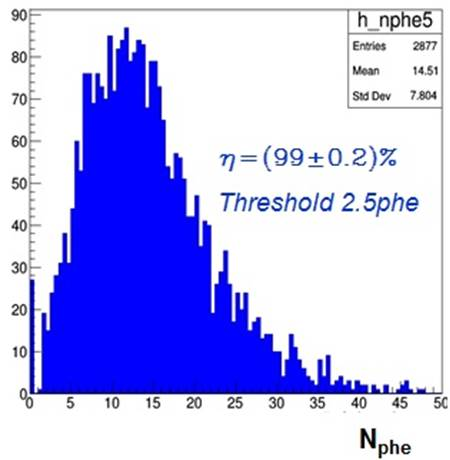
\includegraphics[width=1.0\linewidth,trim={0.0cm 0.0cm 0.0cm 0.0cm},clip]{images/RAFO_2GeV.jpg}
    \caption{Rejection of charged pions at 4 GeV}
    \label{fig:RAFO_2GeV}
\end{figure}

The corresponding thresholds applied were approximately 2.5 phe. Measurements were performed using a special procedure with a random trigger which was not correlated with the HTCC. There were observed 27 events not detected by HTCC due to threshold. As shown, the electron detection efficiency is $\eta$ = (99$\pm$0.2) \% which is in good agreements with the MC estimate. This result can be considered as a conservative estimate.

On the Fig.\ref{fig:positivePNPEC6595} response of the detector in the wide range of particle momentum. The increase of number of events at high momenta is due to registration of charged pions and this is clearly illustrated.

\begin{figure}[!ht]
    \centering
    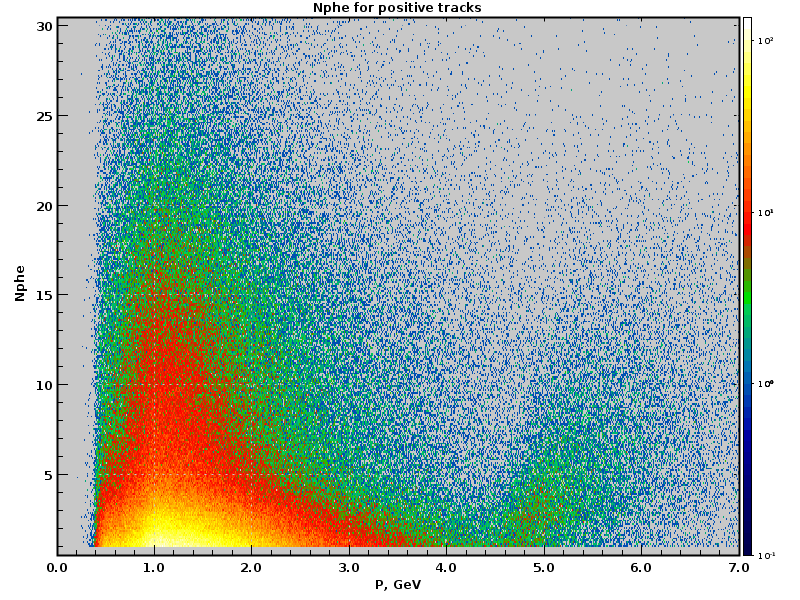
\includegraphics[width=1.0\linewidth,trim={0.0cm 0.0cm 0.0cm 0.0cm},clip]{images/positivePNPEC6595.png}
    \caption{Distributions of the HTCC response in wide momentum range including region beyond threshold of charged pion registration}
    \label{fig:positivePNPEC6595}
\end{figure}
As shown bellow in the Fig.\ref{fig:avgNPE_Theta_Phi_Dev_Build-2_NO_HOLES} the signal strength goes up for the utmost mirrors (large electron scattering angles). This is because electrons travel a longer distance in the radiator gas (10\% to 30\% difference depending on angle.) In other words the electron detection efficiency obtained for elastically scattered electrons at 2 GeV can be considered as as a conservative estimate for the efficiency of electron detection at larger angles. 

\indent The signal strength in the HTCC depends on the actual properties of mirror facets, such as its final shape, reflectance. Accuracy of the combined mirror assembly and of alignment of components (mirror, photomultiplier tubes), the composition of the radiator gas are all influence on final results. The FADC histogram of  typical signal strength distribution obtained in one half-sector \#1 and \#2 of Sector I is shown in the Fig.\ref{fig:Signal_S1_HS1_HS2_R1_R2}

\begin{figure}[!ht]
    \centering
    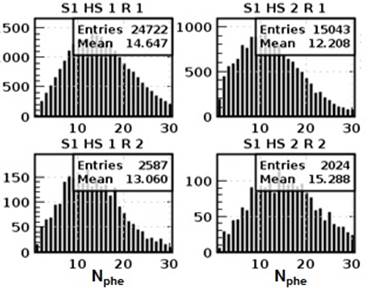
\includegraphics[width=1.0\linewidth,trim={0.0cm 0.0cm 0.0cm 0.0cm},clip]{images/Signal_S1_HS1_HS2_R1_R2.jpg}
    \caption{Typical distributions of signal strength in channels covering polar angles in range of $5^\circ$ to $12.5^\circ$ (Ring 1) and $12.5^\circ$ to $20.0^\circ$ (Ring 2) within azimuthal interval of $60^\circ$}
    \label{fig:Signal_S1_HS1_HS2_R1_R2}
\end{figure}
The signal strength for scattered electron event averaged over all HTCC channels are is brought on the Fig.\ref{fig:Average_HTCC_Signal}. As on can see the experimentally measured mean value of 16.3 phe is close to Monte-Carlo simulation results, see Fig.\ref{fig:10cm_Targ_5T_Field_Phi}.

\begin{figure}[!ht]
    \centering
    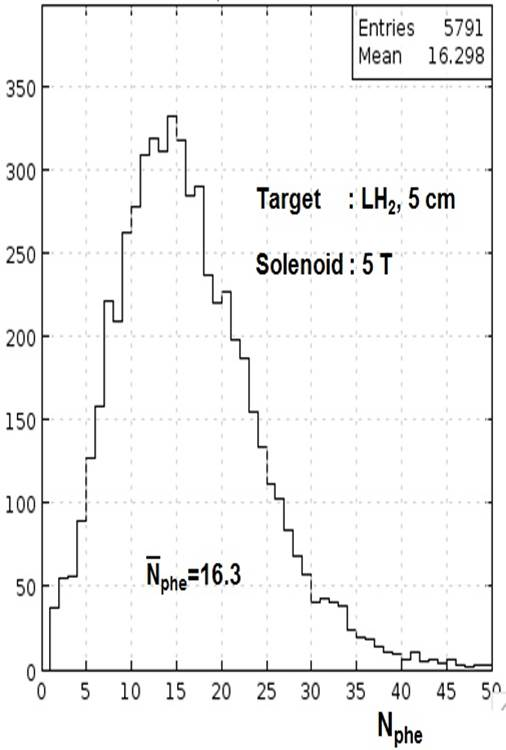
\includegraphics[width=1.0\linewidth,trim={0.0cm 0.0cm 0.0cm 0.0cm},clip]{images/Average_HTCC_Signal.jpg}
    \caption{The HTCC average signal strength of electron detection event}
    \label{fig:Average_HTCC_Signal}
\end{figure}
On the Fig.\ref{fig:HTCC_Response_run4013} 2-dimensional distribution on the HTCC response for electrons is shown.
\begin{figure}[!ht]
    \centering
    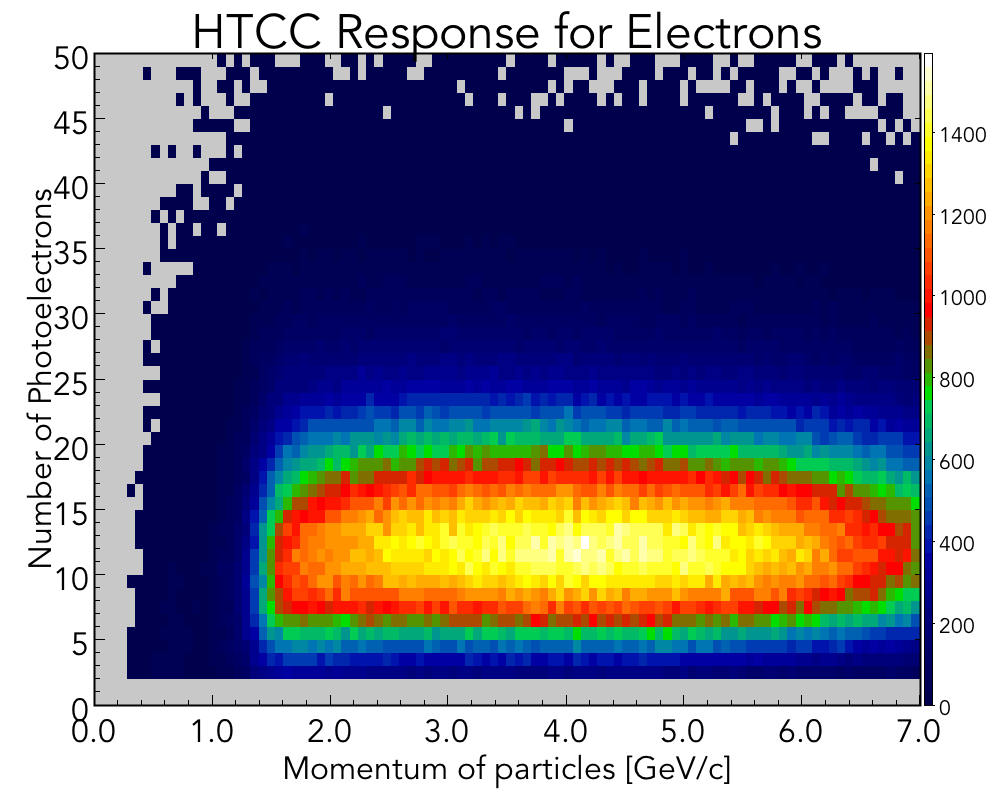
\includegraphics[width=1.0\linewidth,trim={0.0cm 0.0cm 0.0cm 1.73cm},clip]{images/HTCC_Response_run4013.png}
    \caption{The HTCC response for electrons: signal strength vs momentum}
    \label{fig:HTCC_Response_run4013}
\end{figure}
On next  Fig.\ref{fig:avgNPE_Theta_Phi_Dev_Build-2_NO_HOLES} is shown distribution of the HTCC response over the entire face of the mirror in XY-plane.
\begin{figure}[!ht]
    \centering
    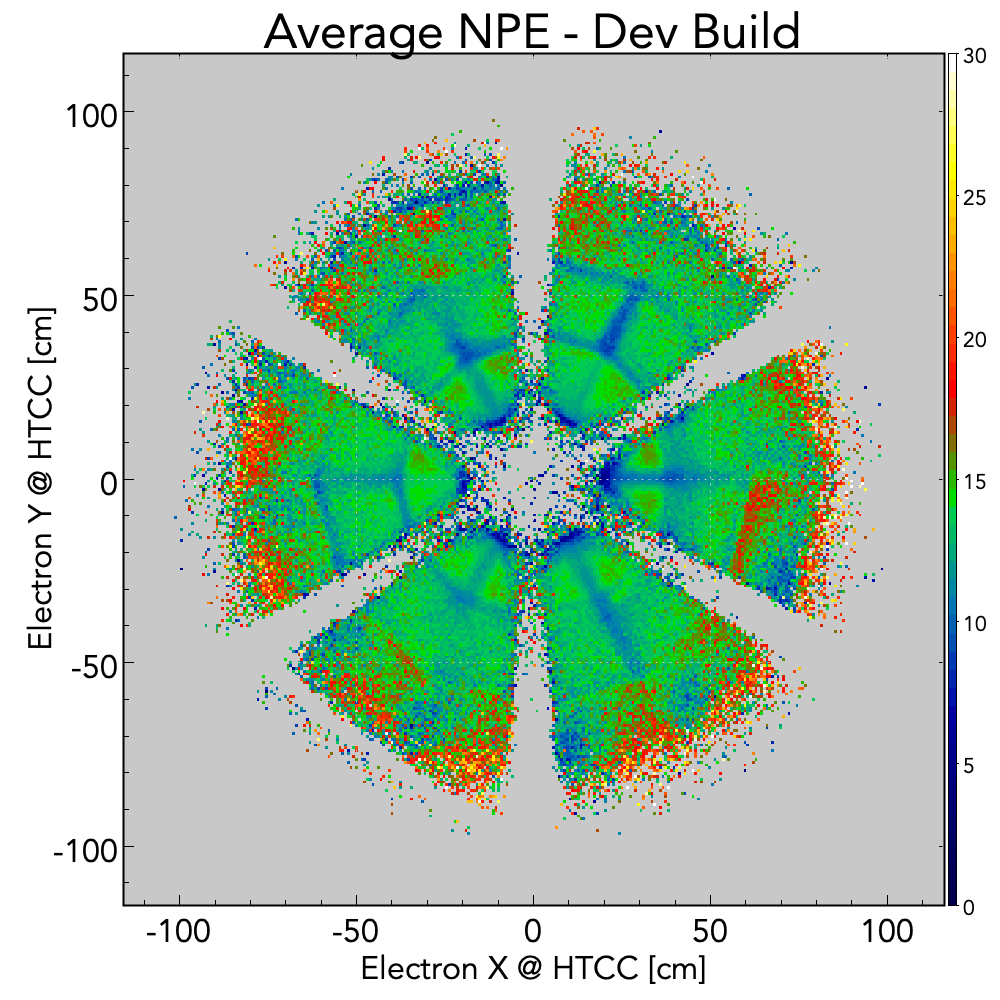
\includegraphics[width=1.0\linewidth,trim={0.0cm 0.0cm 0.0cm 1.67cm},clip]{images/avgNPE_Theta_Phi_Dev_Build-2_NO_HOLES.png}
    \caption{The HTCC response (in $N_{phe}$) for electrons in XY-plane of the mirror}
    \label{fig:avgNPE_Theta_Phi_Dev_Build-2_NO_HOLES}
\end{figure}
Similar distribution is shown on the Fig.\ref{fig:avgNPE_XY_Dev_Build_02npe} obtained at threshold of 0.2 phe.
\begin{figure}[!ht]
    \centering
    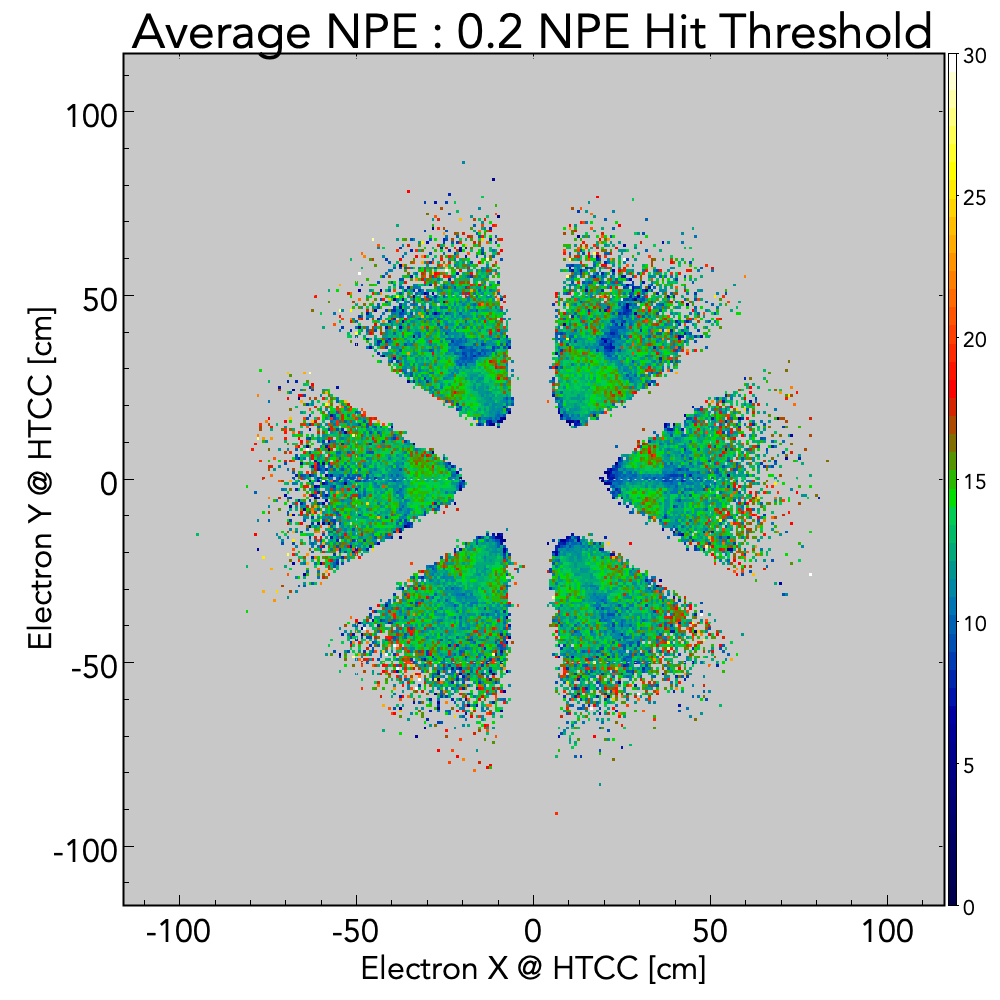
\includegraphics[width=1.0\linewidth,trim={0.0cm 0.0cm 0.0cm 1.67cm},clip]{images/avgNPE_XY_Dev_Build_02npe.png}
    \caption{The HTCC response (in $N_{phe}$) for electrons in XY-plane of the mirror at the threshold of 0.2 phe}
    \label{fig:avgNPE_XY_Dev_Build_02npe}
\end{figure}
Due to the large scattering angles of electrons the statistics are lower in angular range of 27.5$^\circ$ to 35$^\circ$, see Fig.\ref{fig:statistics_Theta_Phi_Dev_Build_NO_HOLES} where are given distribution of statistics in all 6 sectors. Data allows to conclude that the integrated signal strength is about 16.5 phe.
\begin{figure}[!ht]
    \centering
    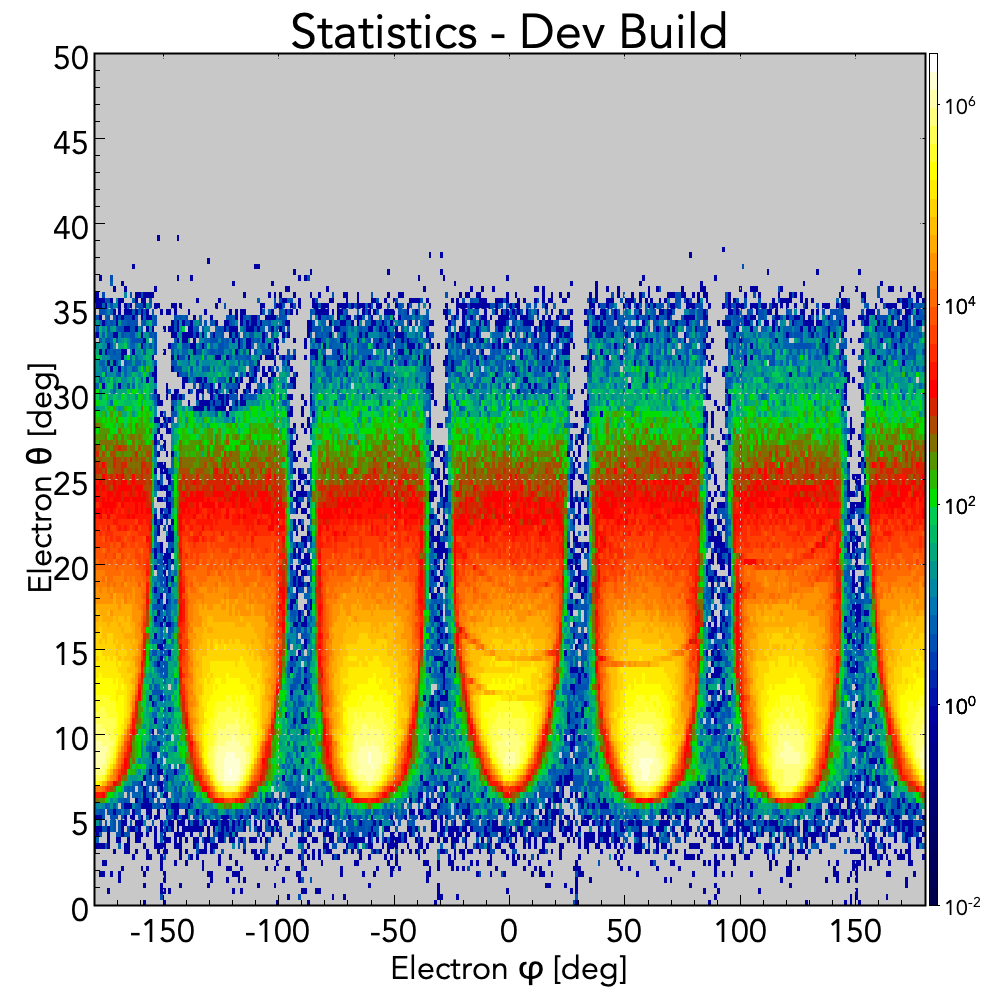
\includegraphics[width=1.0\linewidth,trim={0.0cm 0.0cm 0.0cm 1.67cm},clip]{images/statistics_Theta_Phi_Dev_Build_NO_HOLES.png}
    \caption{Distribution of statistics in 6 sectors}
    \label{fig:statistics_Theta_Phi_Dev_Build_NO_HOLES}
\end{figure}
We also in particular note that in cases when the electrons are crossing the mirror close to its edges (at approximately at
5$^\circ$ and 35$^\circ$) one should expect unavoidable losses in the signal strength: some part of Cerenkov light just passes by the mirror. As far as the “internal” borders between adjacent mirrors is concerned there are are similar losses that of course take place and are finally compensated due to the complete azimuthal symmetry of the detector.\\
\indent As mentioned in subsection 3.4, gluing mirror facets with each other with epoxy glue applied in dots does not change their shape. The overall shape stays unchanged but a mirror gets deformed in the direction normal to the mirror’s face due to shrinkage of the glue. As a result the region along glue joints defuse light impinging the area, i.e. the signal strength is decreasing. The width of that area along boundaries is estimated to be between $\sim$5 to $\sim$10 mm. This area includes technological zone ~0.5 mm of width that is not reflecting the light at all.\\
\indent On the Fig.\ref{fig:avgNPE_Theta_Phi_Dev_Build-2_NO_HOLES} presenting the experimentally obtained signal strength distributions for all 60 mirror facets one can see areas along “internal” borders between adjacent mirror facets where signal strength is lower than average. This edge effect is normal for the given design of the detector. The results can be improved if zero-shrinkage glue is used. 
